\documentclass[a4paper,12pt]{article}
\usepackage[margin=2.5cm]{geometry}
\usepackage{setspace}
\onehalfspacing

\usepackage{array}
\usepackage{multirow}
\usepackage{csquotes}
\usepackage[usenames,dvipsnames]{color}
\usepackage[utf8]{inputenc}
\usepackage{pdfpages}
\usepackage{rotating}
\usepackage{longtable}
\usepackage[labelfont=it]{caption}
\usepackage{color}
\usepackage{soul}
\usepackage{amsfonts}
\usepackage{graphicx}
\usepackage{caption}
\usepackage{subcaption}
\usepackage{eurosym}

\usepackage{titling}
\newcommand{\subtitle}[1]{%
  \posttitle{%
    \par\end{center}
    \begin{center}\large#1\end{center}
    \vskip0.5em}%
}

% Highlight
\definecolor{highlightyellow}{rgb}{1,1,0.7}
\sethlcolor{highlightyellow}
\makeatletter
\newcommand\fix{%
  \let\set@color\beamerorig@set@color
  \let\reset@color\beamerorig@reset@color}
\makeatother

% Note and Source below tables and figures
\usepackage{threeparttable}% Alternative for Notes below table
\newcommand{\Figtext}[1]{%
	\begin{tablenotes}[para,flushleft]
		\hangindent=1em
		\footnotesize
		\raggedright
		#1
	\end{tablenotes}
}
\newcommand{\Fignote}[1]{\Figtext{\emph{Note:~}~#1}}
\newcommand{\Figsource}[1]{\Figtext{\emph{Source:~}~#1}}

% TITLE PAGE
\title{\Large {\bf Auction or haggling -- what should the seller choose?} \\ A look at the interaction between learning and competition in Name-Your-Own-Price auctions.}
\subtitle{(Third draft)}
\author{Jonas K. Sekamane}
\date{18. December 2014\thanks{This paper is written for the seminar \emph{Experiments in Economics} at the Department of Economics, University of Copenhagen in the autumn 2014. I would like to thank the participants, my supervisor Ulrik Haagen Nielsen and opponent Aksel Thomsen for their questions and comments.}}

% NEW COMMANDS AND TYPES
\newcolumntype{x}[1]{%
>{\raggedright\hspace{0pt}}p{#1}}%


\begin{document}
	
	\pagenumbering{gobble}% Remove page numbers
	\clearpage
	\thispagestyle{empty}
	
	\maketitle{}
		
	\newpage
	
	\clearpage %  Reset page numbers to 1
	\pagenumbering{arabic}
	\setcounter{page}{1}
	
	\begin{abstract}
		{This paper investigates the optimal design choice when selling a single and unique item (such as art, antiques, or collectibles). The paper compares and discusses three price mechanisms: the posted price mechanism, the Name-Your-Own-Price (NYOP) mechanism and the English auction. The first and novel contribution of this paper is the introduction of the NYOP mechanism under supply constraints. The paper proposes a lab experiment that will rank the revenue of the NYOP and the English auction. This comparison of revenue is the second novel contribution of the paper. Additionally the experiment will investigate how the NYOP is affected by competition among buyers and by buyers learning the seller's threshold level. Therefore the experiment focuses on the behaviour of buyers. The third novel contribution of the paper is how competition and learning affect behaviour.}
	\end{abstract}
	
	%\tableofcontents
	
	%\newpage

	\section{Introduction}

	Which price mechanism should the seller choose? This article focuses on the selling of unique objects or scarce goods, i.e. where multiple buyers compete for the same object. And so the seller is in essence a monopolist. This area has traditionally been the realm of auctions (art, antiques, collectibles, second-hand, etc). But perhaps -- and contrary to popular believe -- the standard single-item auction formats are not the optimal selling methods. An alternative price mechanism is the Name-Your-Own-Price (NYOP). In NYOP the seller sets a posted price and commits to threshold level. Then a buyer proposes a price (bid). If the proposed price is above the threshold level, then the buyer gets the object at his or her proposed price. As shown later, the NYOP can in some cases be though of as haggling. Haggling and bargaining is usually used to accommodate buyers with low values (Neeman el. at 2013 p.609). Bargaining can imposes high haggling costs on the seller. The seller can lower his or her exposure to this cost, by allocating the bargaining power to a third party (eg. marketplace or shop assistant). However this in turn opens for principal–agent problems. Advances in information technology has significantly mitigated these problems and costs, such that haggling, and in particular the NYOP, has found its way back into the arena (Terwiesch et. al. 2005 p.339).
	
	All the three price mechanisms are used to sell unique items. DBA.dk, the largest second-hand marketplace in Denmark, officially uses a posted price mechanism. But looking through the comments, one quickly realises that haggling takes place frequently. While Lauritz.com, the largest Danish online auction house, sells using a slightly modified English auction. And finally auctionata.com, the largest German online auction house, uses both auctions and NYOP. The NYOP is used for items valued below \euro300.000. \emph{Why are all three mechanisms prevalent? Why choose one mechanism over the other for low-valued items? If haggling only accommodates buyers with low values, why then use the NYOP to sell single and unique items? Why not officially embrace and improve upon the price mechanism unofficially chosen by sellers and buyers alike?} It is questions like these that have motivated my research into the three mechanisms. The paper will not directly try to answer these questions. It requires other considerations since the marketplaces also differ in inventory, segments, layout, organisational structure and politics, etc. Instead the paper will focus on how the prices mechanisms affect the behaviour of buyers.
	
	A previous experiment by Shapiro and Zillante (2009) shows that NYOP gives the seller a higher revenue than a simple posted price mechanism when there is no constrain on supply. To my knowledge no previous articles on NYOP constrains the supply. Instead there is an item for every buyer, and hence no competition among buyers (see figure~\ref{fig:competition-items}). The lab experiment proposed in this paper tries to answer, if using a NYOP can give the seller a higher revenue than an English auction. But before this, the paper introduces competition into the NYOP, such that it is in fact comparable to the competition found in auctions.  Secondly the experiment tries to understand why -- why revenue is higher in NYOP, or why revenue is not higher? To explain this and the resulting differences between auctions and NYOP, I will compare the main NYOP treatment to three alternative NYOP treatments. In total the experiment will be composed of five treatments (see figure~\ref{fig:treatments}). These are henceforward referred to as $AUCTION_0$, $NYOP_0$, $NYOP_P$, $NYOP_S$, and $NYOP_M$, where the control treatment is $NYOP_0$. All the treatments are explain in detail in section~\ref{sec:treatments}. My hypothesis is that in particular two factors effects the results of the NYOP mechanism: learning and competition. The two factors have counteracting effects on revenue. And by appropriately balancing them, the seller can maximise the revenue of the single-unit NYOP. 

	\begin{enumerate}
		\item {\bf Learning} or price discovery: Through experience and information about previously submitted bids buyers will learn and come to form correct expectations about the seller's threshold level. This will, everything else equal, result in buyers submitting bids closer to the threshold and significantly below the posted price, thus having a negative effect on the seller's expected revenue. I identify three separate channels through which learning happens: 1) the \emph{individual channel} where buyers bid repeatedly and incrementally until they reach the threshold level, 2) the \emph{common channel} where buyers observe what others bid and use this to form expectations about the threshold level, and 3) the \emph{experience channel} where buyers, by participating in multiple rounds, learn the winning bid in each round and from this gradually learn the general distribution of the threshold level.
	 	\item {\bf Competition}: I introduce competition into the NYOP by reducing the number of items for sale and using an allocation rule henceforward referred to as First-Come-First-Served (FCFS). There are fewer items than buyers creating scarcity and competition\footnote{Similarly auctions have competition due to scarcity. The allocation rule determines that the buyer with the highest (HIGH) bid wins the item.}. This pressures buyers to submit earlier bids, since only the first bid above the threshold level wins the item. The pressure will, everything else equal, imply that buyers have less time available to discover the threshold level. Hence buyers are not as likely to shade their bids -- or alternatively they disengage from bid-shading, and simply use the `buy' option purchasing the item at the posted price. This will have a positive effect on the seller's expected revenue.
	\end{enumerate}

	This paper is structured as follows. First the prices mechanisms are introduced (posted price, NYOP, haggling, English auction). This section includes a small discussion of how the various price mechanisms relate to one another. Hereafter follows the full description of the experiment: its design, treatments, procedure, participant requirements and expected results. The last sections of this paper includes a recapitulation of my hypotheses, the shortcomings of the experiment, future extensions, and a conclusion.

	\section{Price mechanisms}

	Before diving into the experiment itself, I will set the stage by properly introducing each of the price mechanisms. I will discuss their similarities, introduce notation and concepts. And with this the latter parts of the paper will be more easily understandable.

	\subsection{Posted Price}
	The simplest and most common price mechanism is a posted price (also known as {\it listed price}, or {\it take-it-or-leave-it offer}). You encounter this price mechanism everyday when going to the supermarket or retail shops. Here the seller proposes and sets the price. The price is visible to all. Buyers can only choose to buy the item at the posted price, or choose not to buy. There is often no official count down or time limit on the offer. However the item is usually sold to the first willing buyer. The posted price mechanism is simple, familiar and generally applicable. In addition to these advantages, the seller has full control over the final price. If sellers are risk averse this may be the decisive feature when settling on a price mechanism. The main disadvantage is the lack of a price discovery process. I.e. what is the posted price for the seller? If the seller sets the price too low, the item is sold quickly and rents may not have been fully exhausted. If its set too high, the item is sold slowly or not at all. Often the seller will be uncertain about the value of the item. Perhaps not the seller's own valuation or reserve price, but uncertain about what the highest value is among all potential buyers. This problem is more prevalent when selling a single and unique item, because there is no prior market price that can guide the seller. In addition buyers may value the exclusivity and the uniqueness of the item, far beyond its mere production costs.

	\subsection{Name-your-own-price (NYOP)}

	\begin{figure}
	        \centering
	        \caption{NYOP game tree}
	        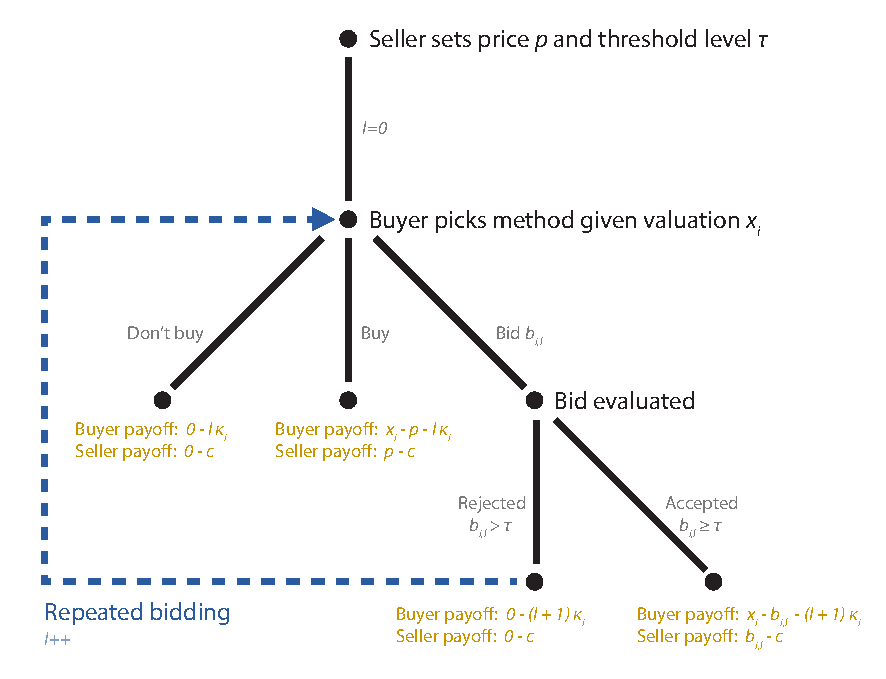
\includegraphics[width=\textwidth]{Figures/NYOP_GameTree}
			\label{fig:game_tree}
			\Fignote{Where $l$ is number of bids attempted, $\kappa_i$ is haggling cost of buyer $i$, $c$ is marginal cost, $\tau$ is threshold level, $p$ is posted price, $x_i$ is value of buyer $i$ and where $b_{i,l}$ is the $l$'th bid of buyer $i$. Here it is assumed that haggling costs are constant and proportional to the number of bids, $l$.}
	\end{figure}

	The name-your-own-price mechanism (also known as {\it reverse pricing} or {\it name-your-own-price auction}) is an extension of the posted price mechanism. The seller decides the posted price and a threshold level at which he or she is willing to sell the item. Only the posted price and the buyer's own value is known to the buyer, who now have one additional option besides `buy', and `don't buy'. The buyers can submit a bid. The bid is rejected if it is below the threshold level. And if above, the bid is accepted and the transaction is made with the buyer. This is the essential parts of the NYOP mechanism, but there exist numerous extensions and modifications. One modification is to hide the posted price, but having less cues about the threshold level reduces the average bid (Shapiro and Zillante, 2009). Clearly presenting the posted price has a sort of anchoring effect\footnote{In the behavioural economics literature the `anchor' generally does not add any relevant information to the agents decision -- yet the irrelevant `anchor' still affects the outcome of the decision. In NYOP the posted price contains relevant information about the threshold level.} or reference price. 
	
	The NYOP mechanism has mostly been studied as a method to curb excess capacity or supply. On the internet Priceline.com has been the pioneer of the NYOP mechanism, selling excess hotel capacity and excess seats on planes (Shapiro and Zillante, 2009). Consequently the literature on NYOP assumes that there are items enough for every buyer willing to purchase. There is no constraint on the supply of items for sale and hence no competition among buyers for the items unlike auctions (Shapiro, 2011).
	
	The NYOP could be further extended by allowing repeated bidding, see figure~\ref{fig:game_tree}. If a bid is reject the buyer can `buy', `don't buy' or `bid' a higher amount. In addition it is normal to assume that buyers endure some non-monetary mental cost or haggling cost from bidding (clicking more buttons, disutility of rejected bid, etc). As Terwiesch et. al. (2005) note this implies that buyers will be balancing between bidding too much, giving the seller additional rents, and bidding too little, possibly enduring further haggling cost. Or worse, in the case of not winning the item, wasting haggling cost. With significant haggling cost, the seller would (indirectly) price discriminates buyers based on their haggling cost. Buyers that are more willing to haggle (lower haggling cost) can archive lower prices and higher payoffs. Terwiesch et. al. (2005) argue that fairness concerns as well as legal constraints prohibit more systematic price discrimination. The seller cannot price discriminate on other parameters. E.g. the seller cannot change the threshold level based on the identity of the buyer, nor change the threshold based on the bidding sequence. Buyers purchasing an item at the same point in time must be charged the same price.

	One advantage of the NYOP is that seller maintains control over the final price. The lowest possible final price will be the threshold level. The other advantage is that the NYOP has a built-in price discovery process. Buyers with values below the posted price, but above the seller's threshold level might purchase an item. Unlike the posted price mechanism, the seller's uncertainty about the value, is less critical since they don't need to select an optimal price point, but select an optimal price range.

	\subsection{Haggling}

	As previously hinted at, the NYOP mechanism is not far from haggling or models of {\it bargaining}. In bargaining 1) agents can enter a mutually beneficial agreement, 2) there is a conflict of interest over the agreement and 3) an agreement cannot be reached without the approval of all agents (Terwiesch et. al., 2005). Bargaining can been formulated as a procedure where agents sequentially make decisions. A distinct difference between haggling and repeated-bidding NYOP is that the seller does not initially set or commit to a threshold level. Instead the seller evaluates each bid as they tick in. Hence the threshold variable $\tau$ is not necessarily constant, but could be a function of the buyer identity $i$, the number of attempted bids $l$, the sellers impatience, and the set of previously submitted bids by other buyers $b_{j,l}$. Often, even in simple bargaining models, multiple equilibria arise.

	The NYOP haggling model proposed by Terwiesch et. al. (2005) assumes that the threshold level is constant. Furthermore it assumes that all uncertainties (other buyers' value, other buyers' beliefs, etc) can be lumped together into a single distribution. This way the problem of finding equilibrium simplifies to a problem of search. In this search problem buyers balance between search efforts (by minimising haggling costs or bids) and choosing a bid that is just above the threshold level (by bidding repeatedly and incrementally until a bid is accepted). A key requirement here, that allows sellers to charge a price above the marginal cost, is that haggling costs are non-zero.

	\subsection{English auction}

	In standard auctions the buyer with the highest bids wins the item. In the English auction bids are open and visible to all. The transaction price is the second highest bid and the buyer does not shade his or her bid, but in theory bids his or her true value. Buyers continue to incrementally outbid each other until there is no challenger, or until the clock runs out. The linkage principle tells us that revenue in the English auction is as least as large as in the second-price auction (Krishna, 2009). There are good theoretical results ranking the revenue of most standard auction formats. And many experimental studies have been carried out trying to confirm these results (Kagel and Levin, 2011). 

	... fewer participants, leads to less competitive arousal or less `frenzy' and that this is what gives lower prices and revenue (more on the latter below when the discovery process is discussed). 

	Sellers can use a secret reserve price, where buyers only know that a reserve price exists, but not its value. Thus when bidding they form prior expectations about the value of the reserve price. When the auction ends the buyer with the highest bid wins, but only if the bid is above the secret reserve price. I mention the reserves price here, since they bear some similarities with the threshold level in the NYOP auction.

	Auctions have many advantages. One is the price discovery process, that may lead to higher expected profits that the posted price mechanism. This is an especially appealing feature when selling scarce goods where the seller is uncertain about the value. Another advantage is that standard auctions are efficient since they allocate the item to the buyer with the highest value (see footnote~\ref{footnote:efficient}). A disadvantage is that the seller has no control over the final price. This may especially be problematic for risk averse sellers. Some solutions to this has been discussed above, such as reserve price or secret reserve price.

	I choose the English auction, firstly because this format has the most features in common with the NYOP, hence it is easier to interpret the results as {\it ceteris paribus}. Secondly, because it has an element of learning and competition build in, which is the main focus of the NYOP treatments. Learning happens in the English auction since bidders can bid repeatedly and see the bids of other buyers. Competition is present in all auctions, because of scarce supply and an allocation rule that says the highest bidder wins the item. Auctions with `hard close' (a fixed, announced end time) often see snipping behaviour. Buyers simply wait until the very last minutes or seconds before they submit bids. The rationale is that by submitting last-minute bids the buyer does not reveal information to other buyers. Often it will be a small subset of sophisticated buyers that engage in sniping. Since I am not interested in studying the snipping behaviour of a subset of buyers, but rather learning and group learning, the experiment will use randomly varying duration also known as a {\it candle auction}.

	\section{Literature review}

This section will review some of the theoretical and experimental results in the literature. The main focus will be on explaining the difference in revenue between the posted price, NYOP, and auction mechanism. And some focus will also be given to learning and competition in the NYOP.


[REWRITE THIS SO FOCUS IS ON LEARNING]
Shapiro and Zillante hypothesis that the fear of buyers learning the threshold level might be the reason why marketplaces have an opaque feature (emphasis added):
\blockquote[Shapiro and Zillante, 2009, p.737]{\emph{ ... Priceline customers are more likely to purchase the same product many times (e.g. a ticket between New York City and Los Angeles) and consequently there is a substantial \emph{\bf risk that customers might quickly learn the threshold range and decrease their bids}. When this is not the case, as at http://www.prisminister.dk which sells consumer electronics, the NYOP website does not have the opaque feature. Indeed, it is simply \emph{\bf less likely that one person would be buying a washer repeatedly and consequently the customer's information about the threshold is less precise} ...}}

[AUCTIONS]
{\bf Buyout auctions} or {\it buy-it-now} price is other modification to auctions that bears similarities with the NYOP mechanism. The buyout option has been popularised by internet marketplaces such as eBay. Besides bidding in the auction as describe above, buyers have the option to purchase the item at the posted price ending the auction before the clock runs out (temporary {\it buy-it-now} option can also be found on eBay, here the {\it buy-it-now} option disappears once the auction receives its first bid). Buyers will choose the buy-it-now option if their time-sensitivity, transaction costs or disutility from not winning the auction is sufficiently large (Haruvy and Leszczyc, 2010). The {\it buy-it-now} price has puzzled researchers since it places a maximum on the expected revenue of the seller. One possible explanation is that, when buyers are risk averse, a carefully selected price under {\it buy-it-now} may increase revenue. It does so by extracting the risk premium buyers are willing to pay to avoid losing the auction (Kagel and Levin, 2011).
%\fix\hl{*** Look more at explanations from buy-it-now literature, since it may also hold the key/answers to why/why not NYOP would outperform Auction ***}

{\bf Duration} of the auction is another important parameter, especially in internet auctions that can stretch over several days. In long-duration auctions the individual buyer takes his or her time-sensitivity or impatience into account when bidding. Secondly, the duration of the auction will affect the discovery process of the auction. If one imagines that the process by which buyers discover the auction is random, then the longer the duration, the more buyers will find and participate in the auction, which should lead to higher revenue. Haruvy and Leszczyc (2010) summaries a field experiment conducted on eBay and at a local auction platform. The experiment finds that on eBay a longer duration results in higher revenue, while the opposite is true at the local auction and both relations are significant. Haruvy and Leszczyc (2010) argue that this is due to the random arrival process at eBay auctions, while the local auction attracts buyers in higher concentrations, by sending out invitations. Therefore longer duration at the local auction does not lead to more participants, but just less competitive arousal and lower revenue. 

This finding touches on when and why a posted price mechanism or a NYOP mechanism might be preferable to a auction. If the arrival time of buyers is long, then a auction with a short time frame is unattractive because of few participating bidders. Empirically evidence show that the expected revenue in auctions decrease as the number of buyers decrease (SOURCE). But an auction with too long a time frame might equally well be unattractive, if it fore instances lowers the competitive arousal of buyers, leading to lower bids or less out-bidding. The seller can set the optimal duration of the auction, but in most cases is seems unlikely that the seller can significantly influence the arrival process of buyers. And hence there may be arrival process (like long arrival times of buyers) where a posted price mechanism or NYOP mechanism is preferable to auctions. Since competition among buyers in these two mechanism rely less buyers interacting synchronously.


%	| Article                           | Mechanism              | Object    | Bidding   | Comments |
%	| -------------                     |:------------- :       | :-----    | :----     | :-----  |
%	| Shapiro and Zillante (2009)       | NYOP, Posted-price    | multiple (no competition)  | single-bid | ... |

	{\bf Posted price vs auctions}
%	> … finding the optimal posted price involves product-category expertise as well as demand and competition research … category expertise is more useful for posted pricing, experienced sellers specializing in a product category should use posted prices more than auction.  

	{\bf Posted price vs NYOP}


	\section{Experiment}

	I will now argue why an experiment is used to investigate auctions and the NYOP mechanism. And why it is not equally or more fruitful to set up models and solve them analytically. There are two main problems with the analytical approach, that one avoids with an empirical or experimental approach. First, the analytical solution often lead to multiple equilibrium or is intractable due to the complexity of the model (see earlier discussion on bargaining models). Secondly, the actual characteristics of buyers and hence their behaviour is vastly unknown. The literature has well established concepts such as `risk aversion' or `anchoring effect' -- but whether, why or when buyers are risk averse remains a mystery in most settings. Haruvy and Leszczyc touch upon these issues in their discussion of traditional auctions vs online auctions:
	\blockquote[Haruvy and Leszczyc, 2010 pp.61-62]{\emph{Traditional auction theory builds heavily on bidder rationality, in many cases risk neutrality, bidder symmetry, revenue and strategic equivalences, and other key properties that are … known to be violated in traditional auction settings as well … In our opinion, based on the research reviewed here, questions of optimal design choice in online auctions can often be addressed empirically and have as much to do with bidder preferences, bidder search, mental processing of information, and issues of trust and reputation as they do with the traditional focus on equilibrium predictions. }}

[Why posted price is not included in experiment]

	\subsection{Design}

	Participants in the experiments will all play the role of buyers. This experiment is interested in studying the behaviour of buyers under different mechanisms. To simplify and control for the behaviour of the seller, the actions of the seller is carried out by a computer. The seller chooses a posted price and threshold level.

	\begin{figure}[h]
	        \centering
	        \caption{Overview of values and distributions}
	        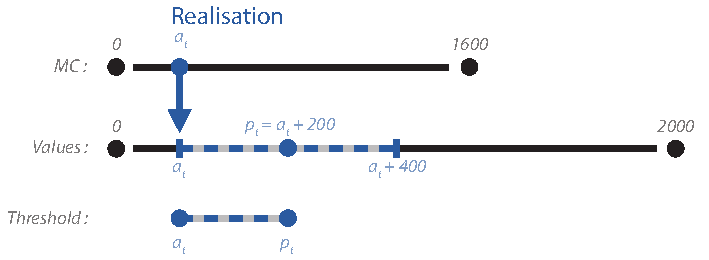
\includegraphics[width=0.7\textwidth]{Figures/Distribution}
			\label{fig:distribution}
	\end{figure}

	In each round, $t$, the values of buyers, the seller's posted price and threshold level are all randomly drawn from uniform distributions, similar to Shapiro and Zillante (2009). In each period the buyers' values are drawn from $U(a_t , a_t + 400)$, where $a_t$ is drawn in each round from $U(0, 1600)$. The lowest value distribution in any round thereby becomes $U(0, 400)$ and the highest $U(1600, 2000)$ and overall values can range between 0 and 2000. Buyers only see their own value and the posted price, they don't receive any information on the distributions. [The posted price is set equal to the expected second highest value of buyers, $p_t = a_t + \frac{N-1}{N+1}400$.] The seller's marginal cost is $a_t$. The threshold level is drawn from $U(a_t, p_t)$. See figure~\ref{fig:distribution}. In the English auction only the buyers' values and posted price is used. There is no reserve price or secret reserve price, but bids have to be strictly positive.
	
	\subsection{Simulation of final price}
	[Each session will have 5 participants ($N=5$).]

	\begin{figure}
	        \centering
	        \caption{Simulation of final price in auction and NYOP for varying number of buyers}
	        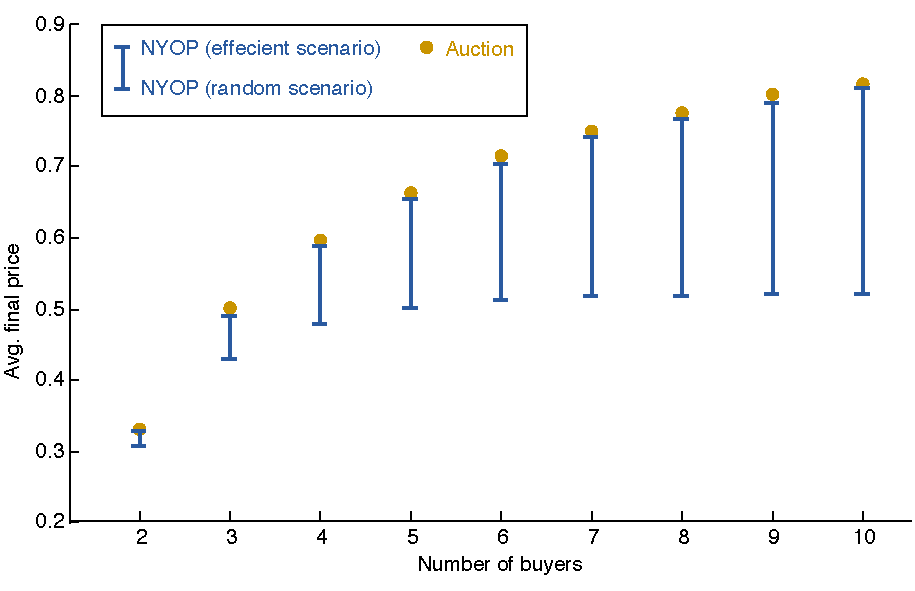
\includegraphics[width=\textwidth]{Figures/FinalPrice_Auction-NYOP}
			\label{fig:FinalPrice_Auction-NYOP}
			\Fignote{Sample size of 10.000. Buyers values are uniformly distributed between $[0,1]$. Second-price auction outcome, e.g. the average value of the second highest buyer. In the NYOP the posted price is the theoretical expected second highest value of buyers: $(\frac{N-1}{N+1})$. Buyers in NYOP are rational such that they only bid if their value is below the posted price, otherwise they `buy' at the posted price. The `efficient scenario' is where the buyer with the highest value manages to purchase the item. The `random scenario' tries to mimic the FCFS allocation rule, in that each buyer is equally likely to purchase the item and the price is therefore the average values of buyers (or posted price). Buyers with values below the threshold level are disregarded in the NYOP.}
	\end{figure}
	
	In second-price auctions the theoretical expected price and expected second highest value among buyers is $\mathbb{E}[Y^{(2)}] = (\frac{N-1}{N+1})$ when values are distributed $U[0,1]$. To my knowledge there is no theoretical or empirical evidence guiding the seller on how to set the optimal posted price in the NYOP mechanism\footnote{The literature instead focuses on the optimal threshold level. From theoretical models Fay (2004) and Terwiesch el. at. (2005) respectively derive the optimal threshold level in the repeated-bidding NYOP. Shapiro and Zillante (2009) set the posted price equal to the monopoly price, but note that it might be sub-optimal. In all three articles they only consider the NYOP under excess supply.}. Under supply constraints it seems logical that the optimal posted price should be increasing in the number of expected buyers, since more buyers increases the likelihood of encountering a buyer with a high value. Given that there are no guidelines to follow when selecting the optimal posted price, I have chosen to set the posted price equal to the expected price in the second price auction. This makes comparisons easy and provides an easily testable hypothesis.

	\emph{Hypothesis 1:} By carefully selecting the posted price, the seller can achieve the same revenue in the repeated-bidding single-unit NYOP as in an English auction. That is $\mathbb{E}[R^{NYOP_0}] = \mathbb{E}[R^{AUCTION_0}]$ when the posted price is set as $P = \mathbb{E}[Y^{(2)}]$.
	
	If the hypothesis above fails I expect the English auction to give a higher revenue than the repeated bidding NYOP. On the other hand, if the hypothesis is true it implies that there might be a range of optimal posted prices above the expected second highest value, $P \in (\mathbb{E}[Y^{(2)}], \bar{P})$, for which the NYOP mechanism outperforms the English auction. And that it could be with in reach if the seller has a fairly good estimate of the number buyers and the distribution of their values. The experiment would provide no information on the upper limit on this optimal posted price range, $\bar{P}$, but leaves this question open for future research.
	
	[More on simulation figure, explain now that its not in the appendix]

	\subsection{Treatments}
	\label{sec:treatments}

	\begin{figure}
	        \centering
	        \caption{Overview of the five treatments}
	        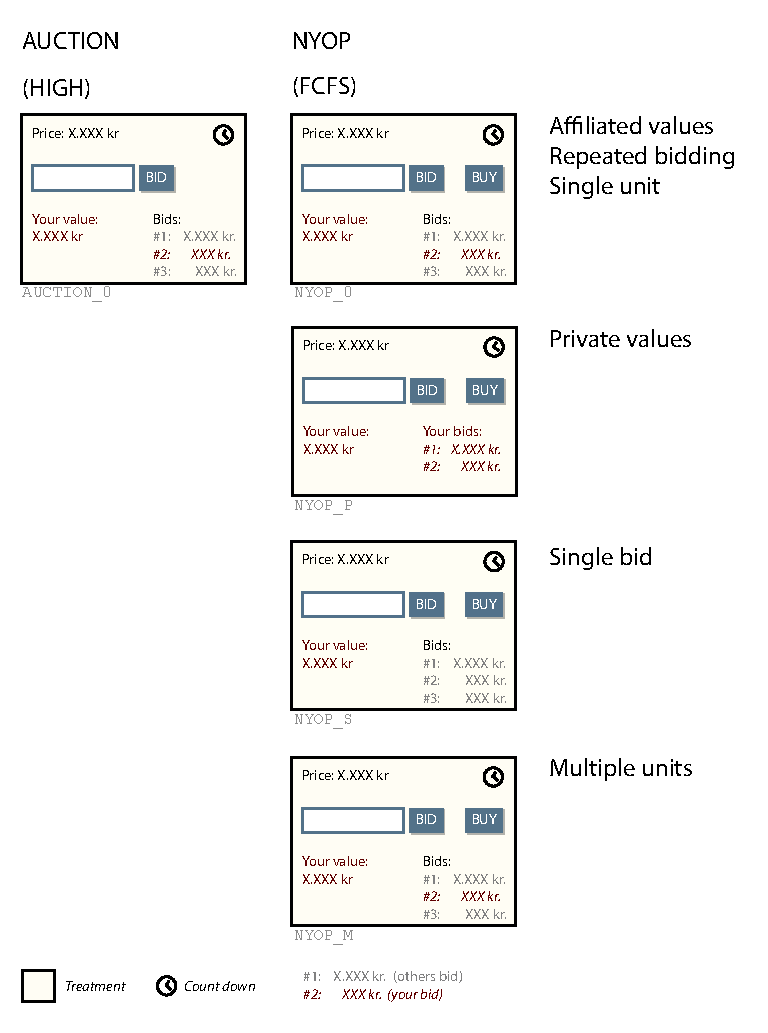
\includegraphics[width=\textwidth]{Figures/Treatments}
			\label{fig:treatments}
	\end{figure}

	There are five treatments see figure~\ref{fig:treatments}, referred to as $AUCTION_0$, $NYOP_0$, $NYOP_P$, $NYOP_S$, and $NYOP_M$. The $NYOP_0$ treatment is the control. The two main treatments are: English auction ($AUCTION_0$) and NYOP ($NYOP_0$).
	In both buyers can repeatedly submit bids (repeated bidding). In the auction buyers can submit a higher bid out-bidding others or themselves. The auctions ends when the clock runs out, and the winner is the highest bidder. In the NYOP a buyer can `buy' or submit a bid, if the bid is above the threshold level, the buyer wins the object and the auction ends. If the bid is rejected, the buyer can `buy' or resubmit a new higher bid. This is the \emph{individual channel} in which learning can happen. The NYOP ends once a buyer uses the `buy' option or once the seller receives a bid above the sellers threshold level. If no one buys and no bids submitted then the NYOP ends when the clock runs out.

	In both treatments all previously submitted bids are visible to all (affiliated values). Buyers can use this information to form and update expectations about the value of other buyers and about the seller's threshold level (in NYOP). This is the \emph{common channel} through which learning can happen. Once the object is sold and the round ends, the posted price along with the winning bid is displayed to all buyers, before the next round initiates. This is done to avoid any confusion about the final selling price, since our interest is learning and how buyers form expectations about the threshold level. Displaying this information hopefully helps us minimise the effects of expectation errors. [\emph{experience channel}].

	In both treatments a single unique unit is put up for sale (single unit). This together with the respective allocation rule introduces competition into both treatments.

	The three additional NYOP treatments, trying to disentangle the counteracting effects of learning and competition, are:

	{\bf Multiple unit treatment} ($NYOP_M$). 
	
	\begin{figure}[h]
	        \centering
	        \caption{Competition and number of items for sale}
	        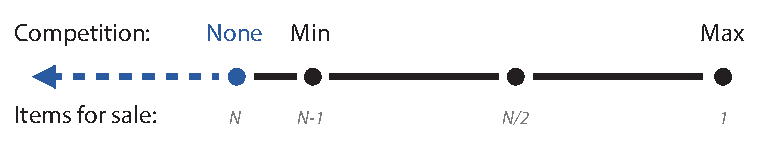
\includegraphics[width=0.7\textwidth]{Figures/Competition-Items}
			\label{fig:competition-items}
	\end{figure}
	
	By selling multiple units rather than a single unit the competition among buyers is reduced, while the learning and price discovery mechanism is unaffected. Winning bids are only displayed after the round ends, while bids below the threshold level are still shown to all. Buyers are not told how many unsold items remain only the total number of units for sale. When the round ends the posted price and all winning bids are shown. [This reason for keeping the prices and number of sold items hidden until after the round ends, is to have the same information as in $NYOP_0$, such that the results in this treatment are not due do buyers receiving extra information.] The number of units to sell in this treatment is somewhat arbitrary (see figure~\ref{fig:competition-items}). A non-arbitrary choice is the same number or more units than there are buyers (excess supply), as this completely eliminates competition. Minimum competition is as attended by selling $N-1$ units, and maximum by selling 1 unit. The multiple object treatment will sell $ceil(N/2)=3$ units. Competition changes in the multi object unit treatment, while learning is unaffected. Compared to $NYOP_0$ changes in revenue will be due to decreased competition among buyers.

	{\bf Single bid treatment} ($NYOP_S$).
	In this treatment buyers are only allowed to submit one bid. If the bid is rejected they cannot resubmit a new nor buy. This restriction removes the buyer's ability to learn the threshold level through the \emph{individual channel} (i.e. by repeatedly submitting incrementally increasing bids until the threshold level is reached). It is still possible to learn through the \emph{common channel}. That is, buyers can still discover the threshold level, but it requires waiting for other buyers to submit their bids, and while waiting they risk that others win the object. And it is still possible to learn through the \emph{experience channel}. The number of buyers might be crucially here, since faced with more competing buyers, one will be more hesitant to wait. Competition among buyers is not affected in the single bid treatment. Changes in revenue will be due to decreased price discovery, e.g. no learning takes place through the \emph{individual channel}.

	{\bf Private value treatment} ($NYOP_P$).
	Another way in which price discovery will change is by restricting the \emph{common channel}. This the the purpose of the private value treatment. Here buyers can only see their own bids. Buyers still have the ability to learn the threshold level though the \emph{individual channel}, but they now have less information about competing buyers. Comparing the results from this treatment with the previous and $NYOP_0$ might help to answer how buyers discover the threshold level -- if it is by individually and repeatedly submitting bids or mainly through observing what others bid. When this treatment removes the option to observe others, do buyers then submit more individual bids? And are they further from guessing the true threshold level? And ultimately what are the effects on revenue? 
	
	\subsection{Procedure of experiment}
	
	Each session has 5 treatments, and 8 rounds per treatment. So each participant goes through a total of 40 rounds. 8 rounds should be enough to uncover learning through the \emph{experience channel}, and not too long, such that it demotivates participants. The duration of each round (in seconds) is drawn randomly from the uniform distribution $U(60, 120)$. Participants will be told that the duration varies, and told that ``each rounds may last a couple of minutes'', but otherwise not be given any information about the distribution and there is no visible countdown. As mention earlier this is done to avoid snipping and encourage early bidding in the auction. The NYOP treatments may end before the clock runs out, if all items have been sold. The order of treatments will vary with session. By varying order one can afterwards test and ensure that the results are not due to a particular ordering (known as spill-over effects). The four last treatment orders have been selected at random, but with the requirement that the auction treatment is either first or last, since different instructions are needed, and to give participants an experience of continuum. Participants will not go through two NYOP treatments, then a auction treatment, and then return to NYOP treatments. Sessions will use one of the five orderings found in table~\ref{tab:order}.

	\begin{table}[ht]
		\caption{Ordering of treatments (randomized)}
		\begin{tabular}{l | l | l | l | l}
			%{\bf a} 	& {\bf b} 		& {\bf c} 		& {\bf d} 		& {\bf e} \\
			$AUCTION_0$	& $AUCTION_0$ 	& $AUCTION_0$ 	& $NYOP_M$ 		& $NYOP_S$ 	\\
			$NYOP_0$ 	& $NYOP_M$		& $NYOP_P$		& $NYOP_P$		& $NYOP_M$	\\
			$NYOP_P$ 	& $NYOP_S$		& $NYOP_M$		& $NYOP_0$		& $NYOP_0$	\\
			$NYOP_S$	& $NYOP_P$		& $NYOP_0$		& $NYOP_S$		& $NYOP_P$	\\
			$NYOP_M$	& $NYOP_0$		& $NYOP_S$		& $AUCTION_0$	& $AUCTION_0$	
		\end{tabular}
		\label{tab:order}
	\end{table}
	
	The experimental procedure is structured as follows: at the beginning of the session participants are given instructions to either the first auction treatment or the first 4 NYOP treatments. Once these treatments are over, the participants are given instructions to the remaining treatment(s). Each new treatment is announced before it begins so participants are aware of the change in environment. At the end of the session two treatments are randomly drawn and participants are paid based on their total earnings in those two treatments (see section about motivation).

	\subsection{Participants: sample size, motivation and incentive problems.}
	Students at the computer lab a University of Copenhagen. Prior knowledge about auctions is not a requirement, nor a impediment to participation. Countless studies have successfully conducted experiments on auctions and competition using students. In regards to the learning effects -- that is how participants come to form expectations about a threshold level that is drawn from an uniform distribution -- requires that participants have no prior knowledge of the distribution. So any participants may take part in only one session.
	
	Participants are given a show-up fee of 50 kr. In addition participants are paid based on their performance. The performance payment is based on two randomly selected treatments of the five treatments. By randomising -- such that participants have no \emph{a priori} knowledge of which exact treatments their payments will be based on -- I hope to keep participants on their toes and engaged throughout the entire session. Hopefully this will lead participants to behave true to their nature, prevent boredom or malicious behaviour. In addition this payment schedule makes it easy for participants to convert values and prices observed in the experiment into danish kroner. Thereby hopefully strengthening the relation between actions in the experiment and the final monetary payment. The performance payment is calculated as the one-tenth of the differences between the buyer's values and the transaction prices (posted prices or bids) for the items that the buyer successfully purchases. The payment is zero in the rounds were the buyer does not manage to purchase an item. This could happen if the buyer's value is below the threshold level, if the buyer is slower than other buyers, or if an other buyer outbids in the auction. Table~\ref{tab:payment} provides examples illustrating how a buyer's payment would look in four different rounds.
	
	\begin{table}[ht]
		\caption{Examples illustrating a buyer's payment at the end of each round}
		\begin{tabular}{p{0.47\textwidth}  p{0.47\textwidth}}
			{\bf Example 1} (NYOP): 	& {\bf Example 2} (NYOP):  		\\
			Value of buyer: 200 		& Value of buyer: 400 			\\
			Threshold level: 300 		& Threshold level: 300 			\\
			Posted price: 450 			& Posted price: 500 			\\
			The buyer does not manage to purchase the item. His/her payment is 0 kr. & The buyer is first and bids 350 thereby purchasing the item. His/her payment is $\frac{400-350}{10}=5$ kr. \\
			\multicolumn{2}{c}{} \\
			{\bf Example 3} (NYOP):  	& {\bf Example 4} (Auction): 	\\
			Value of buyer: 600 		& Value of buyer: 600  			\\
			Threshold level: 300  		& Posted price: 500  			\\
			Posted price: 500  			&  								\\
			The buyer is first and purchases the item at the posted price. His/her payment is $\frac{600-500}{10}=10$ kr. & The buyer bids 550 and the highest competing bid is 450. The buyer wins the item. His/her payment is $\frac{600-450}{10}=15$ kr. \\
		\end{tabular}
		\label{tab:payment}
	\end{table}
	
	The expected payments for one round are 17 kr. and 41 kr. for treatment $AUCTION_0$ and $NYOP_M$ respectively. The expected payments are 14 kr for the treatments $NYOP_0$, $NYOP_S$, $NYOP_P$. See calculations in the appendix~\ref{app:expected_payment}. In each session, when there is 8 rounds per treatment, and taking acount of the combinatorics, a participant can therefore expect a total payment of $50 + \frac{(17+14)3 + (17+41) + (14+14)3 + (14+41)3}{10}8 = 50 + 320 = 370$ kr. While the expected performance payment is quite high so is its variance, since 4 participants gets zero in every round (in four of the treatments).

	Sample size
	
	Motivation

	\subsection{Evaluating experiment -- interpreting results}
	
	[$NYOP_0$ vs. $AUCTION_0$]
	A comparison of these two treatments determines which mechanism gives the highest revenue. It is also possible to evaluate the efficiency of the two mechanisms\footnote{\label{footnote:efficient}An efficient allocation is when the object is allocated to the buyer will the highest value. This is an important consideration (for instance in government held auctions) where the seller also considers the subsequent surpluses. This could either be the winning bidder's surplus or customers of the winning bidder. This article is more aimed at art or antiques, were efficiency concerns are secondary to revenue concerns.}. However this seems unproductive as the NYOP would most likely be inefficient. Efficiency in the NYOP requires that the buyer with the highest value is fastest to evaluate the posted price, form expectations and the fastest to submit a bid above the threshold level. The FCFS allocation rule in NYOP does not promote efficiency. 
	
As earlier noted Shapiro and Zillante (2009) found that an important factor increasing revenue in the NYOP, was the participation of new buyer that were not able to purchase at the posted price. Whether fewer objects lead to higher revenue, will likewise depend on the fraction of new buyers that manage to acquire the item.

	Learning: 
	- $NYOP_0$: individual, common, experience
	- $NYOP_S$: common, experience
	- $NYOP_P$: individual, experience
	Individual and common can be found by comparing treatments. (Experience can be found by including the round, $t$ as control variable).
	
	\section{Conclusion}
			
	shortcomings of the experiment
	- Sellers behaviour: The optimal threshold level of sellers. Can sellers threshold level actually be through of as drawn from some distribution, where there is a clear connection to value of buyers and the posted price. If sellers, don't commit to a threshold level, but are able to evaluate the bids of buyers, how will this then affect the results.
	
			
	\newpage
	\appendix
	
%\renewcommand{\bibname}{Referencer}
	\begingroup
		\section{Referencer}
		\bibliographystyle{apalike-url}
		\nocite{*}
		\renewcommand{\section}[2]{}%
		\raggedright
		\bibliography{ref}
%		\begin{thebibliography}{10}    
%
%
%		\end{thebibliography}
	\endgroup
	
	\section{Expected payments}
	\label{app:expected_payment}
	
	In a $AUCTION_0$ round is (assuming truthful bidding):
	\[ \mathbb{E}[\mbox{payment if highest bidder}] \times \mbox{Prob}[\mbox{highest bidder}] \] 
	\[  = \left( \mathbb{E}[a_t] + (\mathbb{E}[Y^{(1)}]-\mathbb{E}[Y^{(2)}]) 400 \right) \times \mbox{Prob}[x_i \ge Y^{(1)}] \] 
	\[	= \left( 800 + \left(\frac{N}{N+1} - \frac{N-1}{N+1}\right)400 \right) \times \frac{1}{N} = 173 \approx 17\mbox{ kr.} \]
	
	In a $NYOP_0$, $NYOP_P$ or $NYOP_S$ round is (assuming that the fastest buyer is random, each buyer is equally likely to purchase the item. Truthful bidding. And rationality, e.g no bid above posted price):
	\[ \mathbb{E}[\mbox{payment if fastest bidder}] \times \mbox{Prob}[\mbox{fastest bidder}] \] 
	\[  = \left( \mbox{Prob}[\mbox{Value} \ge \mbox{Expected threshold level}] \times \mathbb{E}[\max\{\mbox{Value}, \mbox{Posted price}\} \right)] \times \frac{1}{N} \] 
	\[  = \left( \mbox{Prob}[x_i \ge \mathbb{E}[\tau]] \times \mathbb{E}[\max\{\mathbb{E}[x_i], p\}]  \right) \times \frac{1}{N} \] 
	\[  = \left( \mbox{Prob}[x_i \ge \mathbb{E}[\tau]] \times ( \mbox{Prob}[\mathbb{E}[x_i] < p] \mathbb{E}[x_i] + \mbox{Prob}[\mathbb{E}[x_i] \ge p] p ) \right) \times \frac{1}{N} \] 
	\[  = \left( \left(1-\frac{N-1}{N+1}\frac{1}{2}\right) \times \left( \frac{N-1}{N} \mathbb{E}[x_i] + \frac{1}{N} p \right) \right) \times \frac{1}{N} \] 
	\[  = \left( \left(1-\frac{N-1}{N+1}\frac{1}{2}\right) \times \left( \frac{N-1}{N} (800+400/2) + \frac{1}{N} \left(800+\frac{N-1}{N+1}400\right) \right) \right) \times \frac{1}{N} \] 
	\[	= 135 \approx 14\mbox{ kr.} \]
	
	In a $NYOP_M$ round when there are $ceil(N/2)=3$ items for sale:
	\[ \mathbb{E}[\mbox{payment if fastest bidders}] \times \mbox{Prob}[\mbox{fastest bidders}] \] 
	\[  = \left( \left(1-\frac{N-1}{N+1}\frac{1}{2}\right) \times \left( \frac{N-1}{N} (800+400/2) + \frac{1}{N} \left(800+\frac{N-1}{N+1}400\right) \right) \right) \times \frac{ceil(N/2)}{N} \] 
	\[	= 405 \approx 41\mbox{ kr.} \]
	
	
	\newpage
	\tableofcontents

\end{document}